\documentclass[11pt,a4paper]{article}

% Packages
\usepackage[utf8]{inputenc}
\usepackage[spanish, es-tabla]{babel}
\usepackage{caption}
\usepackage{listings}
\usepackage{adjustbox}
\usepackage{enumitem}
\usepackage{boldline}
\usepackage{amssymb, amsmath}
\usepackage[margin=1in]{geometry}
\usepackage{xcolor}
\usepackage{enumerate}
\usepackage{hyperref}
\usepackage{graphics, graphicx, float}
\usepackage{titlesec} %\titleformat

% Meta
\title{Inteligencia de Negocio: Práctica 2
	\\\medskip \large Análisis Relacional mediante Segmentación}
\author{José Antonio Álvarez Ocete - 77553417Q \\ joseantonioao@correo.ugr.es}
\date{ \today }

% Custom
\providecommand{\abs}[1]{\lvert#1\rvert}
\setlength\parindent{0pt}
\definecolor{Light}{gray}{.90}
\setlength{\parindent}{1.5em} %sangria

% Subsubsubsection (|paragraph)
\setcounter{tocdepth}{4}
\setcounter{secnumdepth}{4}

\begin{document}	
	
	\maketitle 
	\newpage
	\tableofcontents
	\newpage
	
	\section{Introducción}
	
	En esta práctica veremos el uso técnicas de segmentación para realizar análisis relacional sobre un conjunto de datos dado. En nuestro caso utilizaremos los datos de una encuesta sobre fecundidad \cite{encuesta} realizada por el Instituo Nacional de Estadística (INE). En ella se estudian distintas variables de la vida de una persona que pueden haber tenido influencia en la fecundidad de la misma. \\
	
	En particular, 14556 personas respondieron a esta encuesta con un total de 483 variables. Cabe destacar que este es el primer año en el que la encuesta es realizada también por hombres. \\

	Realizaremos tres casos de estudio. En cada uno nos reduciremos a un subconjunto de las variables proporcionadas por la encuesta, al mismo tiempo que realizamos un filtrado sobre la población. Por un lado esto se debe a que la capacidad de cómputo disponible es reducida. Por otro, la información que podemos obtener a partir de la interpretación de los resultados es considerablemente menor si el número de variables es alto. \\
	
	Para esta práctica se han seleccionado 5 algoritmos que ejecutaremos en cada caso de estudio. Detallamos a continuación los parámetros con los que se ejecuta cada algoritmo en el análisis general de cada caso de estudio, a no ser que se especifique lo contrario:
	
	\begin{itemize}
		\item \textbf{K-means}: 5 clusters (\textit{n\_clusters=5}) y ejecutado 5 veces con distintos centroides iniciales, quedándonos con el mejor resultado (\textit{n\_init=5}).
		\item \textbf{MeanShift}: no forzamos a que se añadan todos los elementos a un cluster (\textit{all\_cluster=False}) e imponemos que el número de elementos de las seeds iniciales sea al menos 3 para reducir el tiempo de cómputo (\textit{min\_bin\_freq=3}).
		\item \textbf{Ward}: utilizamos el algoritmo \textit{AgglomerativeClustering} con parámetro \textit{linkage='ward'} como implementación del algoritmo Ward. Adicionalmente fijamos el número de clusters a 5 (\textit{n\_clusters=5}) .
		\item \textbf{DBScan}: Fijamos \emph{épsilon} a 0.35 (\textit{eps=0.35}) y el número mínimo de elementos en el vecindario para que un punto pueda ser centroide a 5 (\textit{min\_samples=5}).
		\item \textbf{Birch}: Número de clusters fijado a 5 (\textit{n\_clusters=5}) y el \emph{threshold} a 0.1 (\textit{threshold=0.1}).
	\end{itemize}
	
	\section{Casos de estudio}
	\subsection{Caso 1: Estudio de los hijos deseados}
	
	En este primer caso estudiaremos principalmente el número de hijos del encuestado en función de las siguientes variables:
	
	\begin{itemize}
		\item \textbf{NHBIOADOP}: Número de hijos que ha tenido el encuestado, ya sean biológicos o adoptivos.
		\item \textbf{EDAD}: Edad del encuestado.
		\item \textbf{NTRABA}: Tiempo que lleva el encuestado en su empleo actual, en años.
		\item \textbf{TEMPRELA}: Tiempo de relación con la pareja actual, en años.
		\item \textbf{NHOGAR}: Tiempo que el encuestado lleva viviendo en el hogar actual, en años.
	\end{itemize}

	Adicionalmente realizamos un filtrado de la población para estudiar unicamente a las personas actualmente empleadas (utilizando \textbf{TRABAJAACT}) para que la variable \textbf{NTRABA} sea lo más relevante posible. Filtramos también aquellos objetos con más de 10 hijos o más de 7 años en el mismo hogar. Estos elementos eran principalmente \emph{outlayers} que complicaban la visuzalización. Con ello reducimos nuestra población a un total de 9161 individuos.
	
	\subsubsection{Análisis general}
	
	En primer lugar ejecutamos todos los algoritmos sobre nuestro conjunto de datos. Presentamos a continuación un resumen de los resultados obtenidos. \\
	
	\begin{table}[H]
		\centering
		\caption{Caso 1: Resultados generales}
		\label{resultados1}
		\begin{tabular}{lllll}
			Algoritmo & Calinski-Harabasz & Silh & Tiempo & Número de clusters \\
			KMeans    & 3871.90 & 0.25 & 0.40   & 5                   \\
			MeanShift & 660.81  & 0.19 & 186.14 & 2                   \\
			Ward      & 2979.72 & 0.17 & 2.50   & 5                   \\
			DBScan    & 11.74   & 0.49 & 1.29   & 2                   \\
			Birch     & 3026.56 & 0.17 & 0.44   & 5                  
		\end{tabular}
	\end{table}

	Antes de analizar los clusters obtenidos miramos los tiempos de ejecución de cada algoritmo para observar como el tiempo de ejecución del algorimto \emph{MeanShift} es absurdamente alto. Ya que no proporcionamos valores para el \emph{bandwidth} ni para las seeds del algoritmo, éste las estima, disparándose el tiempo de ejecución. \\ 
	
	A continuación miramos los resultados obtenidos por el \emph{DBScan}. A pesar de que obtiene el menor valor del coeficiente \emph{Calinski-Harabasz} entre todos los algoritmos, el coeficiente Silhouette es es el mejor de todos, también con diferencia. Este nos hace pensar que el agrupamiento realizado puede ser desigual. Para comprobar esta hipótesis representamos los tamaños de los clusters (en tanto por ciento) para cada algoritmo. \\
	
	\begin{figure}[] 
		\centering
		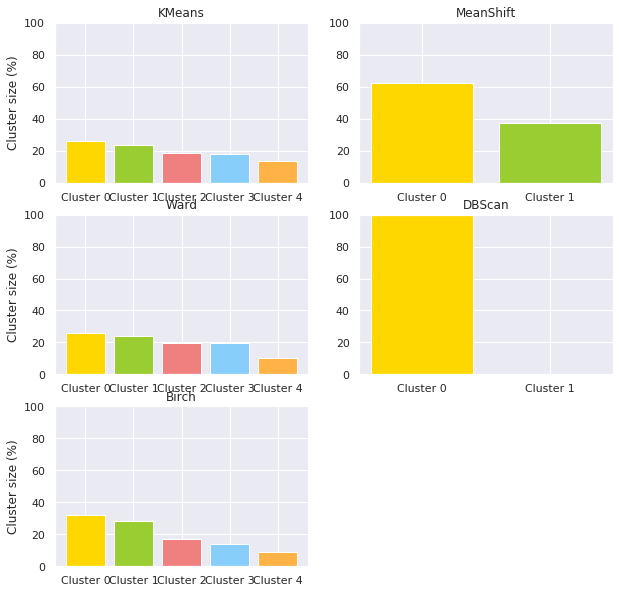
\includegraphics[scale=0.4]{../Caso1/clusters}
		\caption{Caso 1: Tamaños de clusters} \label{clusters1}
	\end{figure}
	
	Observamos en la figura \ref{clusters1} la desigualdad en la distribución comentada con anterioridad. En el caso de \emph{DBScan}, practicamente todos los datos (un 99.98\%) se agrupan en un único cluster, resultando en un alto valor del coeficiente \emph{Silhouette} y un terrible valor para \emph{Calinski-Harabasz}. \\
	
	Los resultados de \emph{MeanShift} son relativamente parecidos. Al no forzar la inclusión de todos los elementos en algún cluster, el algoritmo detecta un 37.49\% de elementos que no sabe clasificar. Estos elementos son el cluster número 1. \\
	
	Respecto a los otros tres algoritmos, obtenemos resultados similares, tanto para el coeficiente \emph{Calinski-Harabasz} como para el \emph{Silhouette}, obteniendo \emph{KMeans} valores algo mejores en ambos. Obviamente el número de clusters obtenido es 5, ya que habíamos fijado tal número como parámetro. \\
	
	Realizamos un estudio paramétrico sobre los distintos algoritmos, excluyendo a \emph{MeanShift} debido al alto tiempo de cómputo. En el caso de \emph{DBScan} alteraremos el \emph{épsilon}, mientras que para los otros tres algoritmos modificamos el números clusters. En la figura \ref{bubbles1} representamos las distintas ejecuciones realizadas, coeficiente \emph{Calinski-Harabasz} respecto al \emph{Silhouette}. Finalmente, el tamaño de cada burbuja indica el valor del parámetro seleccionado en cada caso. En la tabla \ref{tablaComparativa1} se encuentran los resultados obtenidos. \\
	
	\begin{table}[]
		\centering
		\caption{Caso 1: Resultados de ajuste de parámetros} \label{tablaComparativa1} 
		\begin{tabular}{lllll}
			Algoritmo & Silh  & Calinski-Harabasz & Valor del parámetro & N. clusters \\
			DBScan    & -0.39 & 90.24             & 0.05       & 16          \\
			DBScan    & -0.34 & 241.96            & 0.10       & 20          \\
			DBScan    & 0.20  & 122.09            & 0.15       & 2           \\
			DBScan    & 0.32  & 48.07             & 0.20       & 2           \\
			DBScan    & 0.41  & 43.20             & 0.25       & 2           \\
			DBScan    & 0.43  & 26.39             & 0.30       & 2           \\
			DBScan    & 0.49  & 19.40             & 0.35       & 2           \\
			DBScan    & 0.51  & 11.53             & 0.40       & 2           \\
			DBScan    & 0.57  & 9.16              & 0.45       & 2           \\
			KMeans    & 0.33  & 6148.06           & 2.00       & 2           \\
			KMeans    & 0.26  & 4911.49           & 3.00       & 3           \\
			KMeans    & 0.24  & 4293.59           & 4.00       & 4           \\
			KMeans    & 0.25  & 3871.87           & 5.00       & 5           \\
			KMeans    & 0.22  & 3609.15           & 6.00       & 6           \\
			KMeans    & 0.22  & 3355.72           & 7.00       & 7           \\
			KMeans    & 0.22  & 3187.80           & 8.00       & 8           \\
			KMeans    & 0.23  & 3067.40           & 9.00       & 9           \\
			Ward      & 0.28  & 4147.42           & 2.00       & 2           \\
			Ward      & 0.19  & 3688.62           & 3.00       & 3           \\
			Ward      & 0.19  & 3317.32           & 4.00       & 4           \\
			Ward      & 0.17  & 2979.72           & 5.00       & 5           \\
			Ward      & 0.17  & 2819.62           & 6.00       & 6           \\
			Ward      & 0.16  & 2615.95           & 7.00       & 7           \\
			Ward      & 0.16  & 2493.78           & 8.00       & 8           \\
			Ward      & 0.16  & 2429.35           & 9.00       & 9           \\
			Birch     & 0.29  & 4796.80           & 2.00       & 2           \\
			Birch     & 0.21  & 3350.47           & 3.00       & 3           \\
			Birch     & 0.21  & 2680.54           & 4.00       & 4           \\
			Birch     & 0.17  & 3026.56           & 5.00       & 5           \\
			Birch     & 0.17  & 2668.37           & 6.00       & 6           \\
			Birch     & 0.16  & 2381.54           & 7.00       & 7           \\
			Birch     & 0.15  & 2255.30           & 8.00       & 8           \\
			Birch     & 0.13  & 2170.71           & 9.00       & 9          
		\end{tabular}
	\end{table}
	
	\begin{figure}[] 
		\centering
		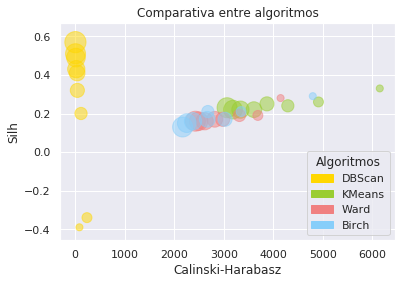
\includegraphics[scale=0.9]{../Caso1/bubbles}
		\caption{Caso 1: Comparativa de parámetros} \label{bubbles1}
	\end{figure}

	Por un lado, el algoritmo \emph{DBScan} obtiene resultados similares independientemente del valor \emph{épsilon}, agrupando los datos a partir de \textit{épsilon=0.15} en dos únicos clusters. Para valores menores que 0.15 se obtienen más clusters, sin llegar a obtener un coeficiente Calinski-Harabasz cercano al del resto de algoritmos. Concluimos por tanto que o bien este algoritmo no es nada adecuado para este subconjunto de individuos debido a la distribución de los mismos, o bien no hemos sabido ajustar los parámetros lo suficiente. \\

	Para el resto de casos, los resultados son consistentes: \emph{KMeans} es el mejor algoritmos para cada valor del parámetro, sin presentar claras mejoras salvo para \emph{n\_clusters=0.2}. Es por ello que procedemos a estudiarlo de forma detallada.
	
	\subsubsection{Análisis específico: algoritmo \emph{KMeans}}
	
	Fijado el algorimto \emph{KMeans} con 5 clusters, representamos el \emph{Scatter Matrix} \ref{scattermatrix1} de los resultados obtenidos, así como el \emph{Heatmap} de centroides asociado \ref{heatmap1}. Procedemos a analizar la distribución en clusters obtenida. \\
	
	\begin{figure}[] 
		\centering
		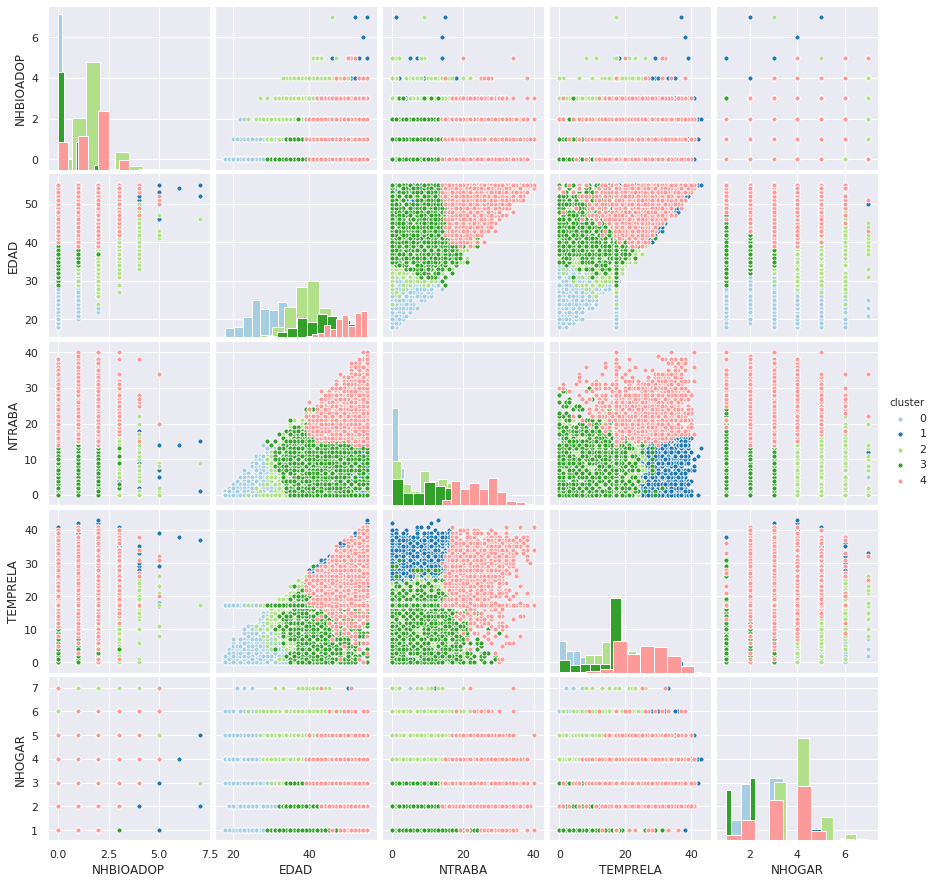
\includegraphics[scale=0.5]{../Caso1/scatter_matrix}
		\caption{Caso 1: \emph{Scatter Matrix} de \emph{KMeans}}
		\label{scattermatrix1}
	\end{figure}
	
	\begin{figure}[] 
		\centering
		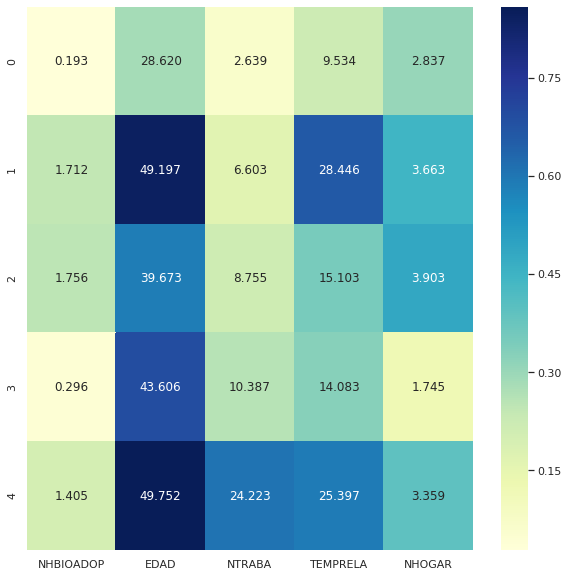
\includegraphics[scale=0.7]{../Caso1/heatmap}
		\caption{Caso 1: \emph{Heatmap} de \emph{KMeans} }
		\label{heatmap1}
	\end{figure}
	
	Por un lado, los dos clusters cuyos encuestados apenas tienen hijos son el 0 y el 3. Además, podemos diferenciar estos claramente en función del resto de variables. En el primero los encuestados tienen entre 20 y 40 años y han estado con su pareja entre 0 y 18 años (10, en media). Además, la mayor parte de este grupo lleva muy poco tiempo en su trabajo, como podemos apreciar en la casilla central de la figura \ref{scattermatrix1}. Entendemos entonces que este cluster esta formado por gente joven, con relaciones relativamente cortas. \\
	
	El cluster 3 es prácticamente opuesto. La edad de sus individuos oscila entre 35 y 60 años, y sus relaciones han sido mucho más duraderas: de 18 a 40 años. Aunque el rango temporal en el que han permanecido en el mismo trabajo es similar al del grupo anterior, de 0 a 18 años, la media es considerablemente mayor, 10.39 años frente a 2.64. Podemos afirmar por lo tanto que este grupo se compone de personas mayores, con relaciones mucho más duraderas y que apenas han tenido hijos. \\

	Llegado este punto cabe destacar como la variable \textbf{NHOGAR} apenas es significativa, como se observa en la figura \ref{heatmap1}. Los clusters toman valores parecidos en dicha variable, resultando curioso que el cluster recién descrito es aquel con menor media (1.75). \\
	
	Comparemos a continuación los clusters 1 y 4. Ambos tienen media de edad parecida y bastante alta, entorno a los 50 años. De la misma forma, ambos grupos llevan viviendo entorno a 3.5 años en su hogar y han tenido, en media, un número de hijos parecido. El factor determinante para diferenciarlos es el tiempo de permanencia en su empleo actual. El cluster 4 tiene una media de 25 años, donde ninguno de sus individuos baja de 17. Estos son los valores más altos de toda la población. Por otro lado, el cluster 2 tiene una media de 6.6 años, tomando valores distribuidos pero aún así claramente diferenciados de los del cluster anterior. \\
	
	Caracterizamos por lo tanto ambos clusters por componerse de gente mayor que han tenido entorno a uno o dos hijos. Diferenciándose entre si por el tiempo de permanencia en su empleo actual. \\
	
	Finalmente, podemos distinguir fácilmente el cluster 2 mirándo unicamente a las dos primeras variables. El número de hijos es relativamente elevado, diferenciándose del primer subgrupo (los clusters 0 y 3), pero cuya edad es, en media, diez años inferior a la del segundo subgrupo (los clusters 1 y 4). \\

	Antes de terminar con este análisis podemos observar en la figura \ref{clusters1} como la segmentación de la población obtenida es relativamente heterogénea, teniendo el cluster 0 casi el doble de individuos que el 4. \\	
	
	\subsection{Caso 2: Análisis jerárquico sobre tratamientos de reproducción asistida. }
	
	En este segundo caso de estudio buscamos realizar un análisis de los métodos jerárquicos. En particular analizaremos un algoritmo de cluster aglomerativo: \textbf{WARD}. Para ello tomaremos un subconjunto de objetos mucho más reducido que en el caso anterior. Las variables utilizadas han sido las siguientes:

	\begin{itemize}
		\item \textbf{NHIJOS}: Número de hijos del encuestado o su pareja.
		
		\item \textbf{TRAREPRO}: Tipo de tratamiento al que se ha sometido el encuestado. Los posibles valores son:
			\begin{itemize}
			\item 1. Coito programado.
			\item 2. Inseminación artificial.
			\item 3. Fecundación in vitro (FIV) o inyección intracitoplasmática (ICSI).
			\item 4. Gestación subrogada.
			\item 5. Otros tratamientos médicos.
		\end{itemize}
	
		\item \textbf{NMESESTRAREPRO}: Número de meses en tratamiento.
		
		\item \textbf{NEMBTRAREPRO}: Número de embarazos conseguidos.
	\end{itemize}
	
	De cara a obtener información relevante en el caso de estudio decidimos estudiar unicamente a aquellos encuestados que se hayan sometido a algún tratamiento artificial usando la variable \textbf{TRAREPRO}. Adicionalmente eliminamos aquellos objetos con un número de embarazos conseguidos mayor a 6 para visualizar mejor la información. Con ello nos restringimos a 807 individuos. Un número tan bajo nos permitirá visualizar mejor los dendogramas asociados al algoritmo de clustering aglomerativo. \\
	
	\subsubsection{Análisis general}
	
	En primer lugar ejecutamos todos los algoritmos sobre nuestro conjunto de datos. Presentamos a continuación un resumen de los resultados obtenidos. \\
	
	\begin{table}[H]
		\centering
		\caption{Caso 2: Resultados generales}
		\label{resultados2}
		\begin{tabular}{lllll}
			Algoritmo & Calinski-Harabasz & Silh & Tiempo & Número de clusters \\
			KMeans    & 316.74 & 0.27 & 0.02   & 5                   \\
			MeanShift & 92.54  & 0.29 & 3.36   & 6                   \\
			Ward      & 276.24 & 0.25 & 0.03   & 4                   \\
			DBScan    & 15.93  & 0.43 & 0.02   & 2                   \\
			Birch     & 199.59 & 0.23 & 0.09   & 5                  
		\end{tabular}
	\end{table}
	
	Comenzamos observando los tiempos obtenidos. De nuevo, el algoritmo \emph{MeanShift} obtiene un tiempo muy superior a los demás, siendo muy inferior al del caso anterior (186 segundos). Esto se debe lógicamente a la diferencia en el tamaño de la población. \\
	
	Para comprender mejor la distribución en clustering representamos de nuevo el tamaño de los mismos en la figura \ref{clusters2}. Observamos que la distribución es similar a la obtenida en el caso anterior (\ref{clusters1}). Los algoritmos obtienen valores parecidos en el coeficiente Silhouette mientras que respecto al Calinski-Harabasz podemos diferenciar dos subgrupos: valores bajos (\emph{MeanShift} y \emph{DBScan}) frente a valores altos (\emph{KMeans}, \emph{Ward} y \emph{Birch}). Esto encaja con la distribución en clustering representada en \ref{clusters2}, donde \emph{MeanShift} y \emph{DBScan} agrupan la mayoría de los datos en un único cluster. Sin embargo, hemos obtenido valores mucho menores del coeficiente \emph{Calinski-Harabasz} que los que obtuvimos en el primer caso de estudio (\ref{resultados1}). Esto podría deberse a que todas la variables utilizadas en este caso de estudio son discretas. Refutaremos esta hipótesis en el tercer caso de estudio. \\
	
	\begin{figure}[] 
		\centering
		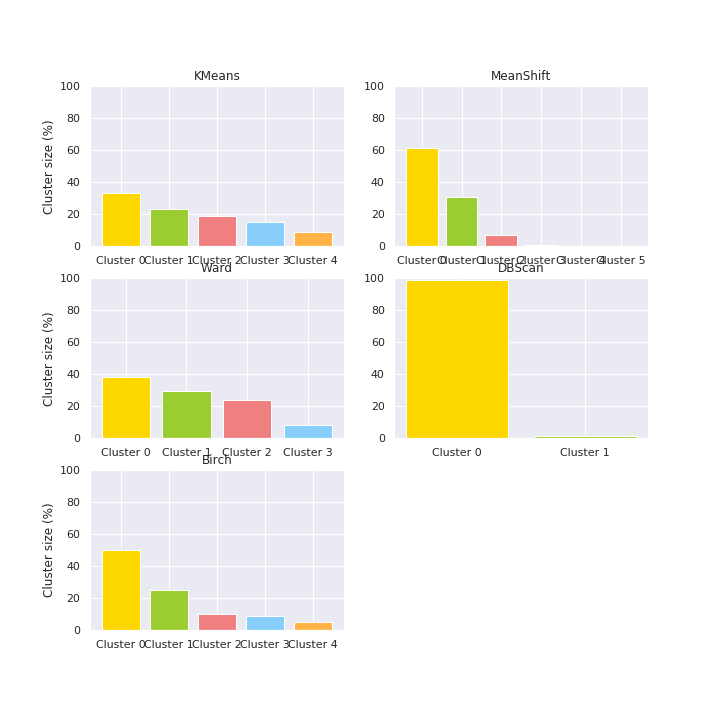
\includegraphics[scale=0.4]{../Caso2/clusters}
		\caption{Caso 2: Tamaños de clusters} \label{clusters2}
	\end{figure}
	
	Pasamos ahora a estudiar los resultados obtenidos por el algoritmo \emph{Ward} en profundidad. 
	
	\subsubsection{Análisis específico: algoritmo \emph{Ward}}
	
	Representamos para cada cluster obtenido un \emph{BoxPlot} de la distribución de cada variable \ref{boxes2}. Visualizamos también un \emph{HeatMap} con los centroides de los distintos clusters \ref{heatmap2}. Debido a que las variables utilizados son todas discretas, la \emph{Scatter Matrix} en este caso de estudio no nos proporciona información relevante. Es por ello que se ha omitido. \\
	
	\begin{figure}[] 
		\centering
		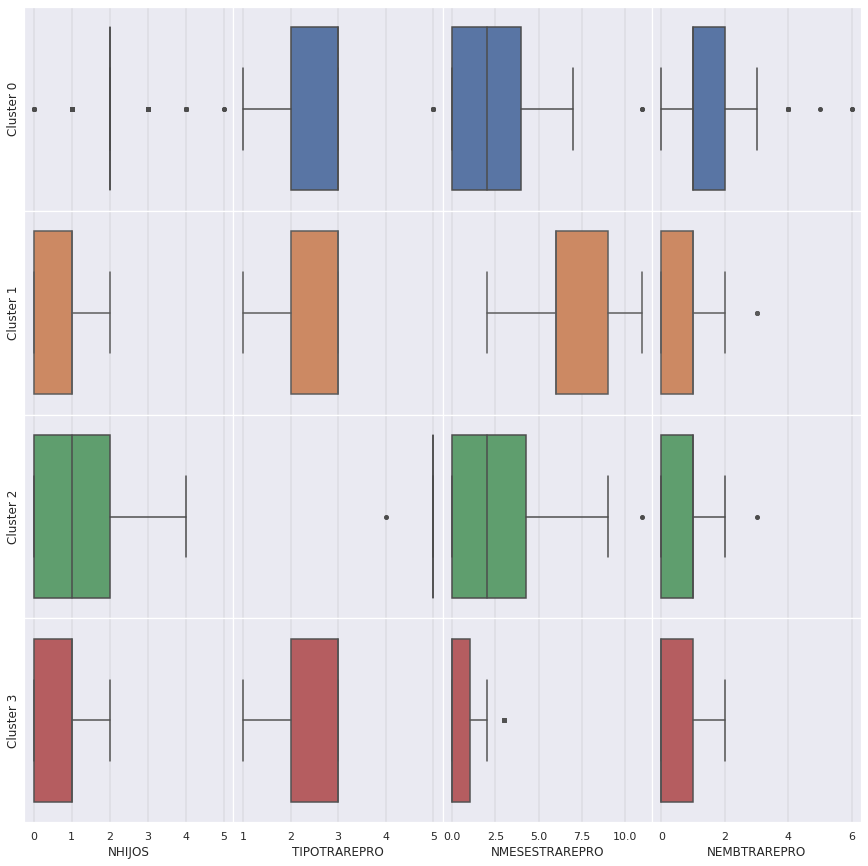
\includegraphics[scale=0.3]{../Caso2/boxes}
		\caption{Caso 2: Distribución de variables en \emph{BoxPlot} para cada cluster} \label{boxes2}
	\end{figure}
	
	\begin{figure}[] 
		\centering
		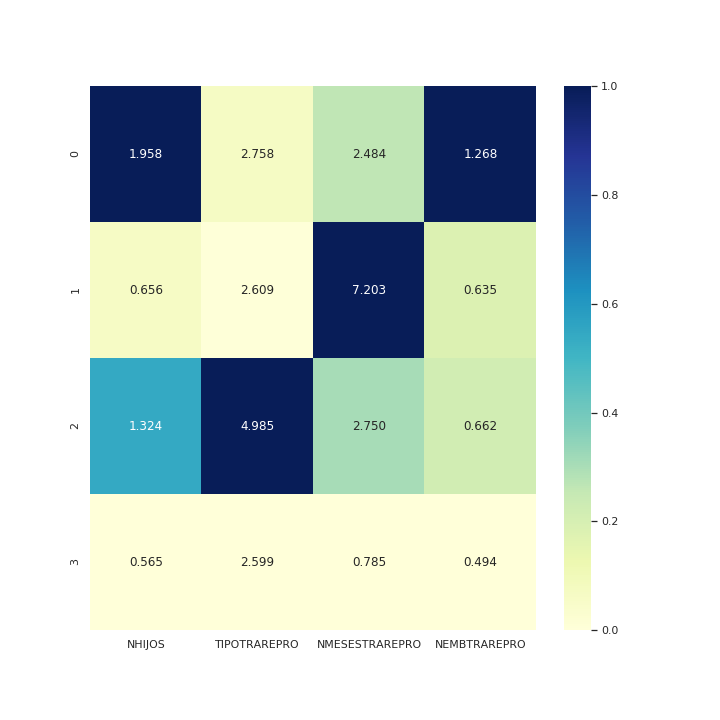
\includegraphics[scale=0.5]{../Caso2/heatmap}
		\caption{Caso 2: \emph{HeatMap} de centroides.} 
		\label{heatmap2}
	\end{figure}

	Los clusters obtenidos son sencillos de analizar mirando la distribución de centroides obtenida en la figura \ref{heatmap2}. Comenzamos fijándonos en el tipo de tratamiento realizado (\textbf{TIPOTRAREPRO}), donde el cluster 2 obtiene un alto valor para el centroide mientras que el resto de clusters tienen valores similares entre si. Comprendemos mejor aún este comportamiento observando la correspondiente columna en el \emph{BoxPlot} \ref{boxes2}. Es claro que se ha agrupado en el segundo cluster aquellos encuestados que respondieron 'Otros tratamientos' a esta pregunta. El resto de clusters toman los valores 'Inseminación artificial' y 'Fecundación in vitro (FIV) o inyección intracitoplasmática (ICSI)', con algunas respuestas de tipo 'Coito programado'. Es posible que esta segmentación fuese distinta si la respuesta 'Otros tratamientos' estuviese asociada al valor 4 en vez de al 5, puesto que no distaría tanto numéricamente de las demás. \\
	
	El cluster 0 se caracteriza por tener altos valores en número de hijos y número de embarazos conseguidos. Si bien estas variables están claramente relacionadas, estudiando ambas buscaba encontrar subgrupos de la población con desbalanceos en las mismas. Por ejemplo, un alto número de hijos y pocos embarazos conseguidos (mostrando parejas que han utiliado métodos de inseminación asistida y han tenido hijos de otras formas), o bajo número de hijos y alto número de embarazos conseguidos, mostrando un alto índice de aborto o situaciones similares. Esto se ha manifestado parcialmente en el cluster dos, dándose el primer ejemplo mencionado. \\
	
	El cluster 1 se caracteriza por presentar un alto valor en meses de tratamiento. Aqui la diferencia es sustancial: siete meses respecto a los uno o dos obtenidos en el resto de clusters. Sin embargo esto tampoco repercute de forma especialmente positiva en el número de embarazos conseguido. Además, apreciamos en \ref{clusters2} que este cluster representa a un 24\% de la población. Es decir, alrededor de un cuarto de los encuestados requirieron tratamientos notablemente más largo, que el resto, de aproximadamente 5 meses más. \\

	Finalmente llegamos al cluster 3, con un 10\% de la población, obteniendo valores bajos en todas las variables. Caracterizaremos este cluster principalmente por la corta duración de sus tratamientos, apenas un mes en la mayoría de los casos (\ref{boxes2}). No todos los encuestados de este subgrupo obtuvieron resultados positivos, ya que el número de embarazos conseguidos es, en media, alrededor de un medio. \\
	
	\subsubsection{Análisis jerárquico de clustering aglomerativo.}
	
	Pasamos a estudiar un dendograma con un \emph{HeatMap} asociado generado utilizando la librería \emph{Seaborn} (\ref{dendograma2}). \\
	
	\begin{figure}[] 
		\makebox[\textwidth][c]{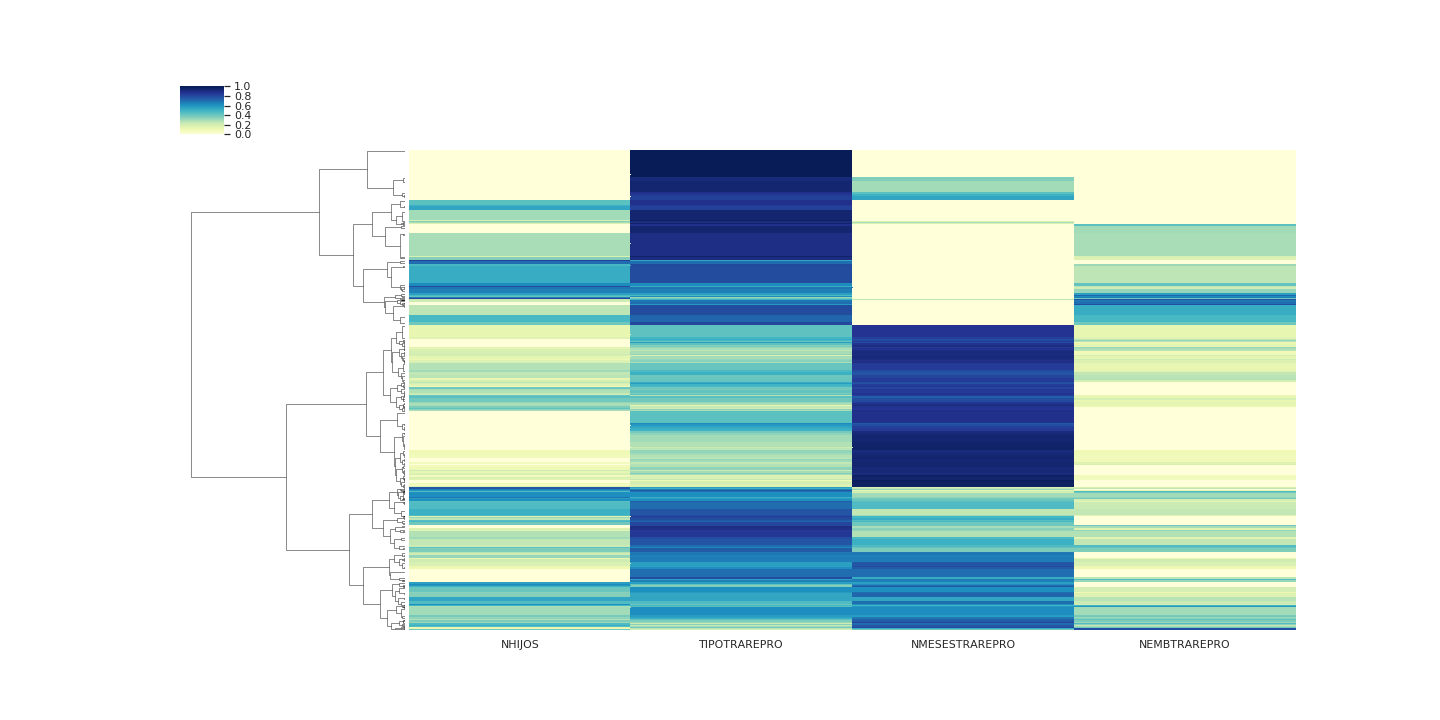
\includegraphics[scale=0.35]{../Caso2/dendograma}}%
		\caption{Caso 2: Dendograma obtenido con la librería \emph{Seaborn}.} 
		\label{dendograma2}
	\end{figure}
	
	He descartado comparar la asociación de clusters estudiada en el apartado anterior añadiendo una columna al dendograma con dicha asociación pues esta no aportaba ninguna información relevante, o al menos que haya podido inferir de la misma. \\
	
	Estudiaremos el dendograma de forma escalonada, viendo las divisiones realizadas de izquierda a derecha, como es natural. \\
	
	Observando la primera división podemos suponer que esta se hace principalmente debido a los altos valores de la variable \textbf{TIPOTRAREPRO} y los bajos valores de \textbf{NMESESTRAREPRO}. Esto es, el tipo de tratamiendo es 'Otros tratamientos' y los tratamientos fueron de corta duración. Podemos relacionar esta segmentación con el cluster número dos del apartado anterior. Denotaremos a este cluster por \textbf{cluster superior}. \\
	
	La segunda división del dendograma divide a la población basándose en la duración del tratamiento. El \textbf{cluster central} agrupa largas duraciones de tratamiento mientras que el \textbf{cluster inferior} contiene duraciones medias: no tan altas como las del cluster central ni tan altas como las del cluster superior. \\

	Hasta ahora las divisiones realizadas unicamente se refieren a la duración del tratamiento y al tipo del mismo. Ante esta segregación podemos suponer que el tipo de tratamiento utilizado por aquellos encuestados que marcaron 'Otros tratamientos' repercute en una poca duración del mismo, ya sea debido a que el tratamiento tiene dicha duración o porque los encuestados deciden dejar de realizarlo. Esta hipótesis dista notablemente de las conclusiones obtenidas en el apartado anterior, donde el cluster 2 recogía a las personas con dicho tipo de tratamiento pero cuyas duraciones eran bajas o medias, no altas (\ref{boxes2}). \\

	Volviendo al dendograma, veamos como los tres clusters comentados se subdividen. Por un lado, el cluster superior se segmenta en basándose en el número de hijos: valores muy pequeños frente a valores intermedios. Llama la antención en esta subdivisión el cluster con encuestados sin hijos y sin embarazos conseguidos. Éste último a su vez se divide dependiendo de la duración de los tratamientos, pero manifiesta esencialmente procedimientos abandonados o fallidos. \\
	
	Caben destacar dos subclusters adicionales del cluster superior. El primero por encajar con una de las conclusiones realizadas en el ejemplo anterior: encuestados con un número de hijos visiblemente superior a número de embarazos conseguidos mediantes tratamientos de reproducción asistida. El segundo por una configuración curiosa de las respuestas obtenidas: Un subgrupo cuyo embarazos conseguidos es superior al del resto de la población y cuya duración de tratamiento es ridiculamente baja. Este cluster se segmenta en otros dos, basado al mismo tiempo en el número de hijos y el tipo de tratamiento. \\
	
	Las divisiones más relevantes en los clusters central e inferior se basan en el número de hijos y la duración del tratamiento respectivamente. El único subgrupo relevante que he podido apreciar está en el cluster central. Se trata de un grupo de encuestados sin hijos y sin embarazos conseguidos cuyo duración de tratamiento es bastante alta. \\
	
	\subsection{Caso 3: Análisis del reparto de tareas familiares en parejas heterosexuales y homosexuales. }
	
	En el último caso de estudio estudiaremos como afecta el reparto de tareas de casa relacionadas con los hijos en las parejas heterosexuales frente a como lo hace en las homosexuales. Comenzamos estudiando unicamente al primer subgrupo. Manteniendo en nuestro conjunto de datos a aquellas parejas Hombre - Mujer (utilizando las variables \textbf{SEXO} y \textbf{SEXOPAR}) que además conviven con al menos un hijo de menos de catorce años (con \textbf{CONVIVEH14}) nos restringimos a un total de 4845 objetos. \\
	
	Cabe destacar que en esta subpoblación, todos los encuestados son mujeres. Aunque esto no era un factor decisivo al decidir el filtrado nos facilitará notablemente el posterior análisis. \\
	
	En la encuesta realizada hay de diez preguntas relacionadas con las tareas de casa que nos interesan particularmente. Son las siguientes:

	\begin{itemize}
		\item \textbf{VESTIR}: Quién viste a los niños.
		\item \textbf{BANAR}: Quién baña a los niños.
		\item \textbf{ACOSTAR}: Quién acuesta a los niños.
		\item \textbf{COMIDAS}: Quién decide la comida de los niños.
		\item \textbf{ENFERMOS}: Quién se queda con los niños cuando estan enfermos.
		\item \textbf{JUGAR}: Quién juega con los niños.
		\item \textbf{DEBERES}: Quién ayuda a los niños con los deberes.
		\item \textbf{COLEGIO}: Quién lleva a los niños al colegio.
		\item \textbf{ROPA}: Quién le compra ropa a los niños.
		\item \textbf{ELIGEEXTRAESC}: Quién elige las actividades extraescolares de los niños.
	\end{itemize}

	% Anulamos la sangría del siguiente párrafo
	{\setlength{\parindent}{0cm} A todas estas preguntas los encuestados podían responder una de las siguientes opciones:}
	
	\begin{itemize}
		\item 1. Entrevistado.
		\item 2. Pareja.
		\item 3. Entrevistado y pareja por igual.
		\item 4. Abuelos.
		\item 5. Otra persona del hogar.
		\item 6. Otra persona de fuera del hogar.
		\item 7. Los niños lo hacen por sí mismos.
	\end{itemize}

	Sintetizaremos la información de todas estas preguntas en un único coeficiente, un valor entre -1 y 1, que denotaremos por \textbf{COEFTAREAS}. Por cada tarea que realice la mujer de la pareja restaremos \emph{0.1} mientras que para cada tarea que realice el hombre sumaremos \emph{0.1}. De cara a entender esta métrica, valores cercanos a cero muestra un equilibro en el repartor de las tareas mientras que valores lejanos denotan un desbalanceo en el mismo. Si el valor es negativo, la mujer está realizando más tareas mientras que si es positivo, lo hace el hombre. \\
	
	Además de este coeficiente utilizaremos las siguientes variables:
	
	\begin{itemize}
		\item \textbf{EDAD}: Edad del entrevistado.
		\item \textbf{NHIJOSCONV}: Número de hijos con los que convive. A pesar de que me habría gustado utilizar \textbf{NHIJOSDESEO} (número de hijos deseado) en su lugar, los 4845 encuestados a los que nos hemos restringido tienen valor \emph{NaN} en dicha variable.
		\item \textbf{ESTUDIOSA}: Nivel de estudios del encuestado. Toma valor en una escala de uno a nueve, donde uno es 'menos que primaria' y nueve, 'enseñanzas de doctorado'.
		\item \textbf{SATISFACENINOS}: Satisfacción del encuestado respecto al reparto de tareas en casa. Toma valor en un escala de cero al diez, donde cero es totalmente insatisfecho y 10, totalmente satisfecho.
	\end{itemize}
	
	\subsubsection{Análisis general}
	
	En primer lugar ejecutamos todos los algoritmos sobre nuestro conjunto de datos, buscando esta vez seis clusters (\emph{n\_clusters=6} para aquellos algoritmos que admiten dicho parámetro). Presentamos a continuación un resumen de los resultados obtenidos. \\
	
	\begin{table}[H]
		\centering
		\caption{Caso 3: Resultados generales}
		\label{resultados3}
		\begin{tabular}{lllll}
			Algoritmo & CH      & Silh & Tiempo & Número de clusters \\
			KMeans    & 1409.53 & 0.20 & 0.18   & 6                   \\
			MeanShift & 971.95  & 0.24 & 44.94  & 2                   \\
			Ward      & 1128.03 & 0.15 & 0.62   & 6                   \\
			DBScan    & 8.11    & 0.41 & 0.46   & 2                   \\
			Birch     & 1024.14 & 0.15 & 0.28   & 6                  
		\end{tabular}
	\end{table}
	
	Observando los tiempos obtenidos vemos como el algoritmo \emph{MeanShift} vuelve a obtener un tiempo absurdarmente alto en comparación con el resto de algoritmos. Uniendo esto a la descomposición de los clusters observada en la figura \ref{clusters3} concluimos que el algoritmo está obviamente mal configurado. Podríamos decir lo mismo sobre \emph{DBScan}. \\

	\begin{figure}[] 
		\centering
		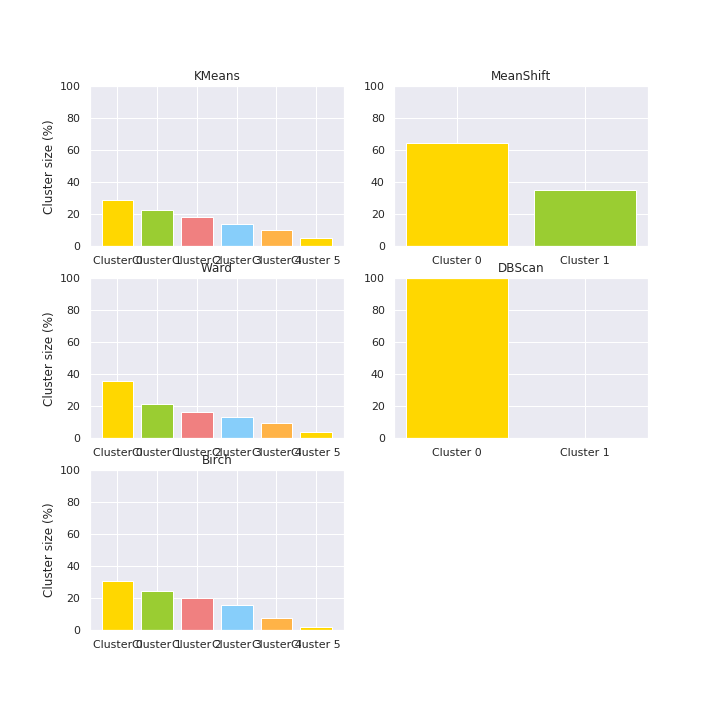
\includegraphics[scale=0.4]{../Caso3/hetero/clusters}
		\caption{Caso 3: Tamaños de clusters para parejas heterosexuales.} \label{clusters3}
	\end{figure}

	Utilizamos la misma estrategia que en el primer caso de estudio (\ref{bubbles1}) para buscar una reconfiguración de los parámetros. Encontramos el resultado en la figura \ref{bubbles3} y la tabla \ref{tablaComparativa3}. Esencialmente se repite el escenario del primer caso de estudio: \emph{DBScan} no genera buenos resultados para ninguno de los valores del parámetro utilizados mientras que los coeficientes Calinski-Harabasz y Silhouette obtenidos por el resto de algoritmos están relativamente agrupados, siendo \emph{KMeans} consistentemente mejor fijando un valor del parámetro. Es por ello que en el análisis específico volveremos a estudiar este algoritmo. \\
	
	\begin{figure}[] 
		\centering
		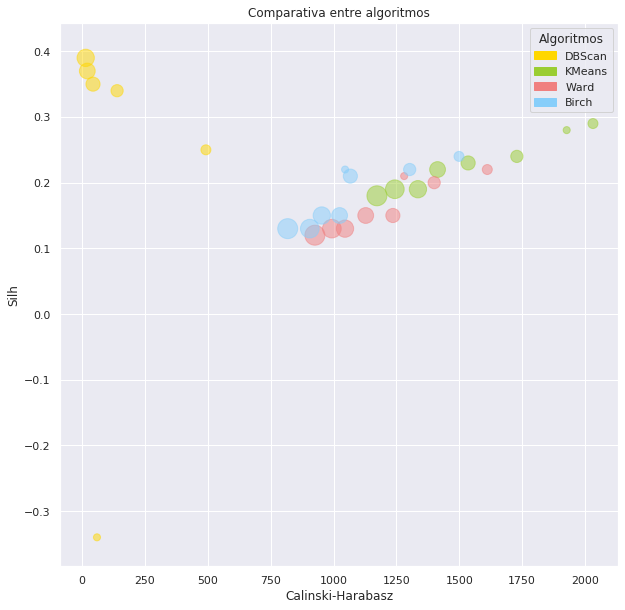
\includegraphics[scale=0.5]{../Caso3/hetero/bubbles}
		\caption{Caso 3: Comparativa de parámetros en parejas heterosexuales.} \label{bubbles3}
	\end{figure}
	
	\begin{table}[]
		\centering
		\caption{Caso 3: Resultados de ajuste de parámetros para parejas heterosexuales} \label{tablaComparativa3} 
		\begin{tabular}{lllll}
			Algoritmo & Silhouette  & Calinski-Harabasz & Parámetro & N. clusters \\
			DBScan    & -0.34 & 59.19             & 0.10       & 13          \\
			DBScan    & 0.25  & 492.42            & 0.15       & 2           \\
			DBScan    & 0.34  & 139.16            & 0.20       & 2           \\
			DBScan    & 0.35  & 43.38             & 0.25       & 2           \\
			DBScan    & 0.37  & 20.70             & 0.30       & 2           \\
			DBScan    & 0.39  & 14.29             & 0.35       & 2           \\
			KMeans    & 0.28  & 1927.36           & 2.00       & 2           \\
			KMeans    & 0.29  & 2031.81           & 3.00       & 3           \\
			KMeans    & 0.25  & 1734.67           & 4.00       & 4           \\
			KMeans    & 0.22  & 1535.91           & 5.00       & 5           \\
			KMeans    & 0.20  & 1409.53           & 6.00       & 6           \\
			KMeans    & 0.19  & 1335.62           & 7.00       & 7           \\
			KMeans    & 0.19  & 1235.59           & 8.00       & 8           \\
			KMeans    & 0.18  & 1168.57           & 9.00       & 9           \\
			Ward      & 0.21  & 1280.85           & 2.00       & 2           \\
			Ward      & 0.22  & 1611.55           & 3.00       & 3           \\
			Ward      & 0.20  & 1400.32           & 4.00       & 4           \\
			Ward      & 0.15  & 1236.06           & 5.00       & 5           \\
			Ward      & 0.15  & 1128.03           & 6.00       & 6           \\
			Ward      & 0.13  & 1045.59           & 7.00       & 7           \\
			Ward      & 0.13  & 993.35            & 8.00       & 8           \\
			Ward      & 0.12  & 925.92            & 9.00       & 9           \\
			Birch     & 0.22  & 1045.99           & 2.00       & 2           \\
			Birch     & 0.24  & 1499.04           & 3.00       & 3           \\
			Birch     & 0.22  & 1302.90           & 4.00       & 4           \\
			Birch     & 0.21  & 1066.88           & 5.00       & 5           \\
			Birch     & 0.15  & 1024.14           & 6.00       & 6           \\
			Birch     & 0.15  & 953.29            & 7.00       & 7           \\
			Birch     & 0.13  & 905.71            & 8.00       & 8           \\
			Birch     & 0.13  & 817.72            & 9.00       & 9          
		\end{tabular}
	\end{table}
	
	Antes de pasar a dicho análisis volvemos a la tabla \ref{resultados3} para descartar una hipótesis formulada previamente. En el segundo caso de estudio atribuimos los bajos valores del coeficiente Calinski-Harabasz proporcionados por todos los algoritmos a la naturaleza de las variables escogidas: todas categóricas. Los valores obtenidos en este caso junto con las variables escogidas nos hace pensar que esto no es cierto. Observando la forma en la que se calcula este coeficiente nos damos cuenta de que depende directamente del número de objetos en estudio, que en el segundo caso era especialmente bajo. Debido a esto obtenemos en este caso de estudio valores intermedios frente a los altos valores del primer caso y los bajos valores del segundo, cuadrando a la perfección con los tamaños de las poblaciones estudiadas en cada caso. 

	\subsubsection{Análisis específico: algoritmo \emph{KMeans} en parejas heterosexuales}
	
	Para este análisis de los clusters obtenidos por el algoritmo \emph{KMeans} generamos una \emph{ScatterMatrix} (\ref{scattermatrix3}), un \emph{HeatMap} (\ref{heatmap3}) y las distribuciones de las distintas variables para cada cluster usando \emph{BoxPlot} \ref{boxes3}. \\
	
	\begin{figure}[] 
		\centering
		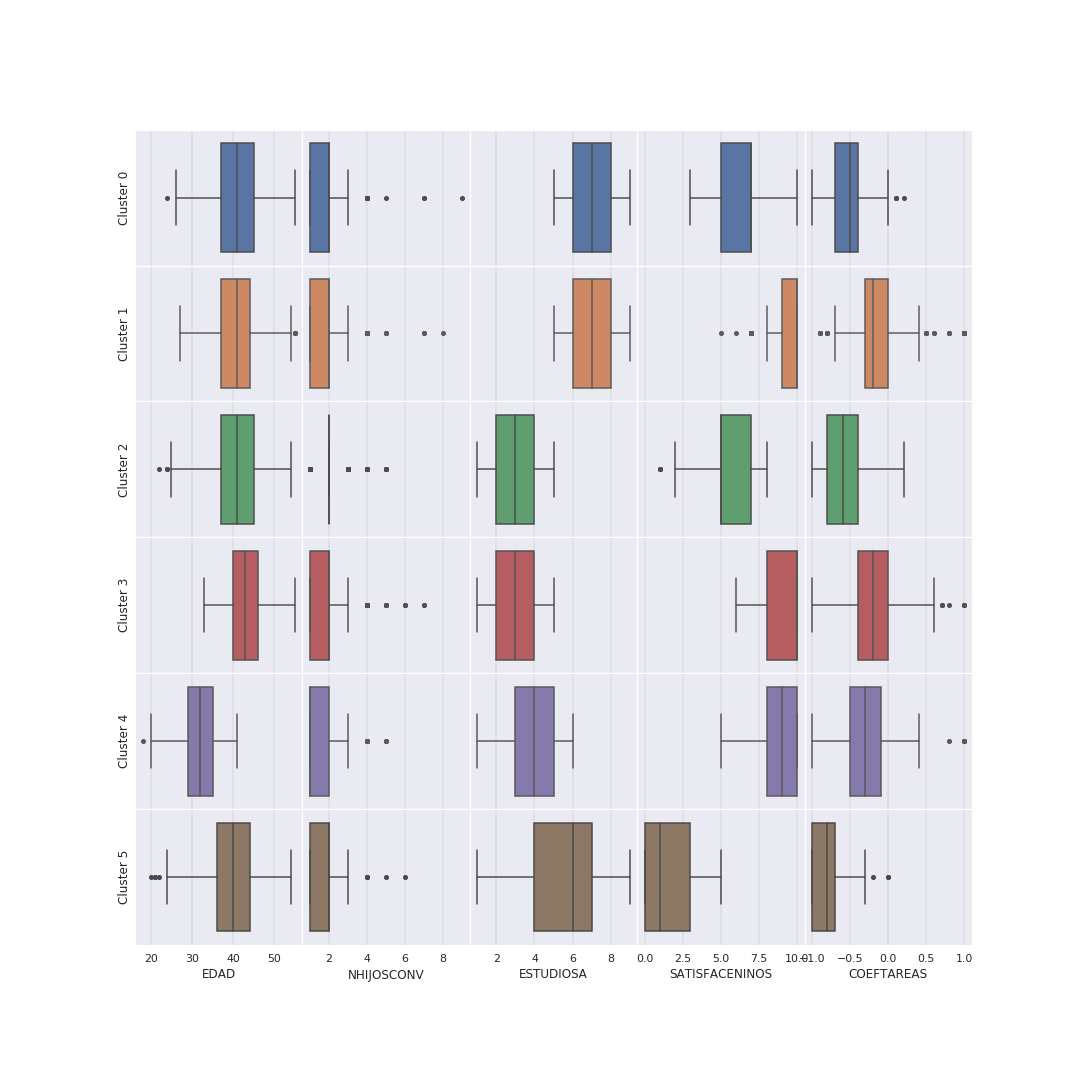
\includegraphics[scale=0.3]{../Caso3/hetero/boxes}
		\caption{Caso 3: Distribución de variables en \emph{BoxPlot} para cada cluster, para parejas heterosexuales.} 
		\label{boxes3}
	\end{figure}

	\begin{figure}[] 
		\centering
		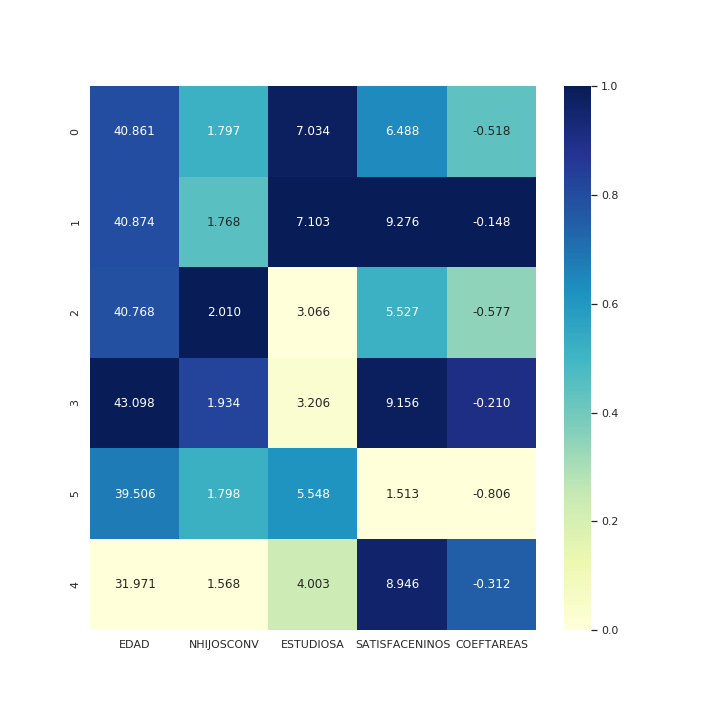
\includegraphics[scale=0.4]{../Caso3/hetero/heatmap}
		\caption{Caso 3: \emph{HeatMap} de centroides para parejas heterosexuales.} 
		\label{heatmap3}
	\end{figure}

	\begin{figure}[] 
		\centering
		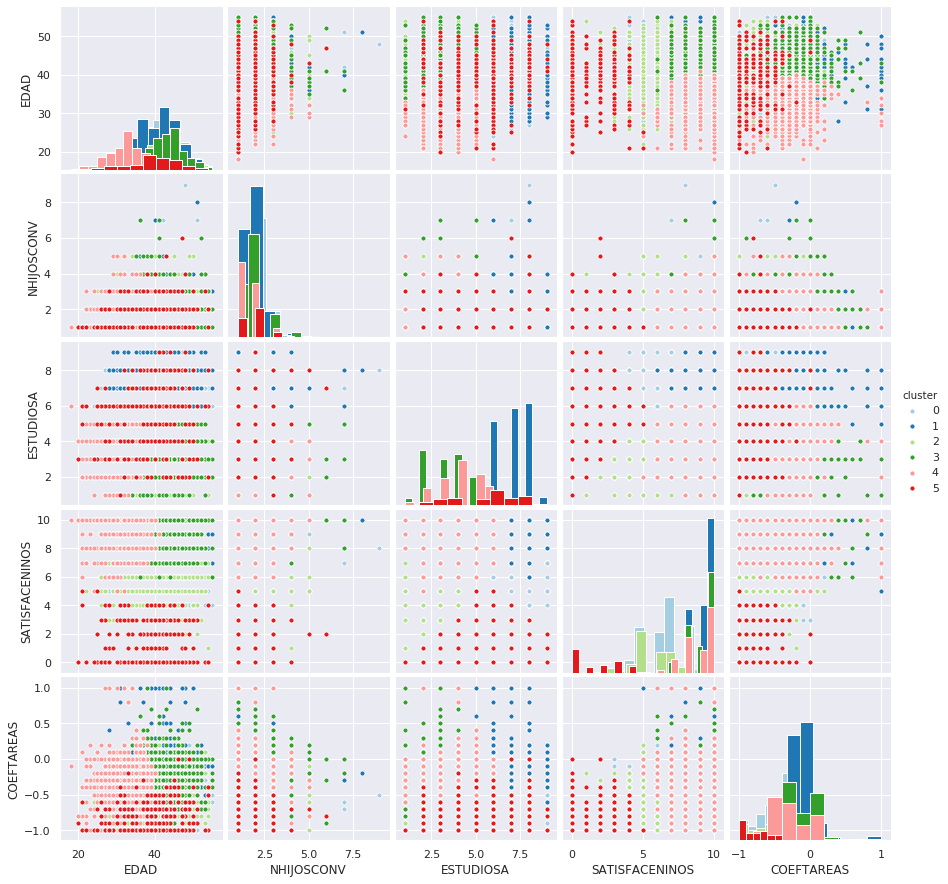
\includegraphics[scale=0.5]{../Caso3/hetero/scatter_matrix}
		\caption{Caso 3: \emph{ScatterMatrix} para parejas heterosexuales.}
		\label{scattermatrix3}
	\end{figure}

	En primer lugar nos fijamos en el coeficiente cálculado sobre el reparto de tareas en la pareja (\textbf{COEFTAREAS}) y la satisfacción de la respectiva encuestada respecto a dicho reparto (\textbf{SATISFACENINOS}). Como es natural podemos observar cierta relación entre las variables. Observamos que en todos los clusters la mujer realiza, en media, más tareas que el hombre. Si bien en algunos clusters esta media es muy cercana a cero y en la figura \ref{boxes3} podemos observar como en algunas parejas si que existe el desbalanceo contrario. \\
	
	En función a estos dos parámetros podemos clasificar los clusters en tres grupos: clusters con bajo (0, 4 y 5), medio (1 y 3) y gran desbalanceo (2). Estudiemos por separado estos grupos. \\
	
	En primer lugar, el cluster 2 es el que más desequilibrio presenta en el reparto. De hecho, observando de nuevo la figura \ref{boxes3}, presenta valores muy agrupados respecto al coeficiente de tareas. La media de edad se situa entorno a 40 años, conviviendo con casi 1.8 hijos y un nivel de estudios medio/alto. Vale la pena remarcar este último hecho: el cluster donde encontramos más descompensación, lo que podría ser signo de un menor nivel de educación, presenta un nivel de estudios relativamente alto. \\
	
	Pasamos a estudiar los clusters con un desbalanceo intermedio (1 y 3). Podemos distinguirlos entre si debido a la abismal diferencia respecto a los estudios alcanzados. El rango de edad y los hijos apenas varían. De hecho, estas dos variables nos dan información relevante en contadas ocasiones de cara a este caso de estudio. Observando \ref{boxes3}, la distribución del número de hijos es practicamente igual en todos los clusters, encontrando más agrupación entorno a dos hijos en el cluster 1. \\
	
	Estudiando finalmente el último subgrupo con un mayor equilibrio en el reparto de tareas (clusters 0, 4 y 5) llegamos al único cluster, el 4, con una diferencia significativa en la edad de los encuestados, entorno a 32 años. También sostiene la menor media en número de hijos, entorno a 1.5, aunque esta varía menos respecto a los demás clusters. Sin embargo, este es uno de los clusters más pequeños (\ref{clusters3}), con unicamente un 10.3\% de los encuestados. Es decir, la mayor parte la subpoblación escogida se sitúa entorno a los cuarenta años. \\
	
	Finalmente diferenciamos los cluster 0 y 5 a partir del nivel de estudios, de igual forma que hicimos con los clusters 1 y 3. Cabe destacar la diferencia de tamaño de los clusters, donde el cluster 0, compuesto por gente con un alto nivel de estudios y un reparto equilibrado, representa el 29\% de la población total mientras que los otros dos clusters con reparto equilibrado suman algo más de un 15\%. Podemos ver como afecta el nivel de estudios a este reparto a partir de estos clusters. \\
	
	A pesar de ello no he obtenido alguno de los resultados que esperaba. En particular esperaba revelar una diferencia entre el reparto de tareas y la percepción del mismo para valores bajos de nivel de estudios. Desconozco hasta qué punto el orden de las preguntas en la encuesta podría haber sugestionado de alguna forma este resultado, y si la respuesta a la satisfacción sobre el reparto de tareas sería la misma si no le precediesen veinte detalladas preguntas sobre el mismo. \\

	En esta ocasión de la \emph{Scatter Matrix} \ref{scattermatrix3} podemos sacar poca información. Debido a la forma en la que está implementada la librería \emph{Matplotlib}, los clusters con mayor número se pinta encima de aquellos con menor número. Es por ello que en dicha figura se observan muchos más valores de los clusters tres, cuatro y cinco a pesar de ser los más pequeños. Esto significa que cuantos más clusters obtengamos, más complicada será la visualización de los mismo utilizando este tipo de gráfica. La única representación que me gustaría descatar en esta \emph{ScatterMatrix} es la representación de \textbf{ESTUDIOSA} frente a \textbf{SATISFACENINOS} (lo que sería la posición \emph{(2,3)} en la matriz), donde vemos una clara segmentación de los seis clusters con las dos variables que más relevantes han sido durante todo el análisis. \\

	\subsubsection{Comparativa con parejas homosexuales}
	
	Realizamos a continuación el mismo análisis que en el apartado anterior para parejas homosexuales. En este caso cambiaremos la forma de calcular el coeficiente de tareas, ya que no tiene sentido estudiar relación Mujer - Hombre en dicho reparto. Para ello realizaremos la misma suma que en el apartado anterior, añadiendo \emph{-0.1} si el encuestado hace la tarea y \emph{0.1} si la hace su pareja. Aplicaremos valor absoluto y obtenemos así un valor entre 0 y 1 donde valores cercanos a 1 representan un desequilibrio en el resparto y valores cercanos a 0, un equilibrio del mismo. De esta forma unicamente tenemos en cuenta el equilibrio en el reparto añadiendo la simetría de este caso de estudio. \\
	
	Nos restringimos por tanto a los 30 encuestados cuyo sexo coincide con el de su pareja y viven al menos con un hijo menor de catorce años. Como hicimos anteriormente, representaremos los resultados del algoritmo \emph{KMeans} mediante una \emph{ScatterMatrix} (\ref{scattermatrix3homo}), un \emph{HeatMap} (\ref{heatmap3homo}), las distribuciones de las distintas variables para cada cluster usando \emph{BoxPlot} \ref{boxes3homo} y los tamaños de los distintos clusters \ref{clusters3homo}. Pasemos a comentar los resultados. \\
	
	En primer lugar, al tratarse de una subpoblación tan sumamente pequeña las conclusiones obtenidas no serán muy representativas de la totalidad población española. Sin embargo, puede servirnos para una comparación con el caso heterosexual. Segmentaremos en cuatro grupos y a pesar del reducido número de objetos obtenemos clusters claramente diferenciados. \\
	
	Podemos apreciar en la figura \ref{heatmap3homo} como los clusters 1 y 3 presentan un gran equilibrio en el reparto de tareas frente al inmenso desequilibro del cluster 2. De hecho vemos una gran concentración de los valores de este último cluster para las variables \textbf{SATISFACENINOS} y \textbf{COEFTAREAS}. \\
	
	Respecto a los clusters 1 y 3, el factor discriminante vuelve a ser el nivel de estudios aunque no de forma tan decisiva como en el caso heterosexual. Ambos clusters se diferencian también en edad y número de hijos. \\
	
	Finalmente el cluster cero, con un 40\% de la población, aglomera parejas con un reparto relativamente desequilibrado (tomando el coeficiente de tareas valores entre 0.25 y 0.75), pero cuya satisfacción al respecto es notablemente alta, concentrándose la gran mayoría de valores en el 8 (\ref{boxes3homo}). \\
	
	Con tan pocos objetos es complicado realizar una comparación eficaz con la segmentación presentada anteriormente. Aunque se realiza un agrupamiento principalmente basado en el reparto de tareas (como era de esperar, ya que dos de las cinco variables están relacionadas directamente con éste), no se aprecia una clara segunda segmentación basada en el nivel de estudios como ocurría para parejas heterosexuales. Si bien el número de clusters es menor y esto permite en menor medida una segunda segmentación, aumentar el número de clusters degeneraba en grupos demasiado reducidos para ser relevantes. \\
	
	\begin{figure}[] 
		\centering
		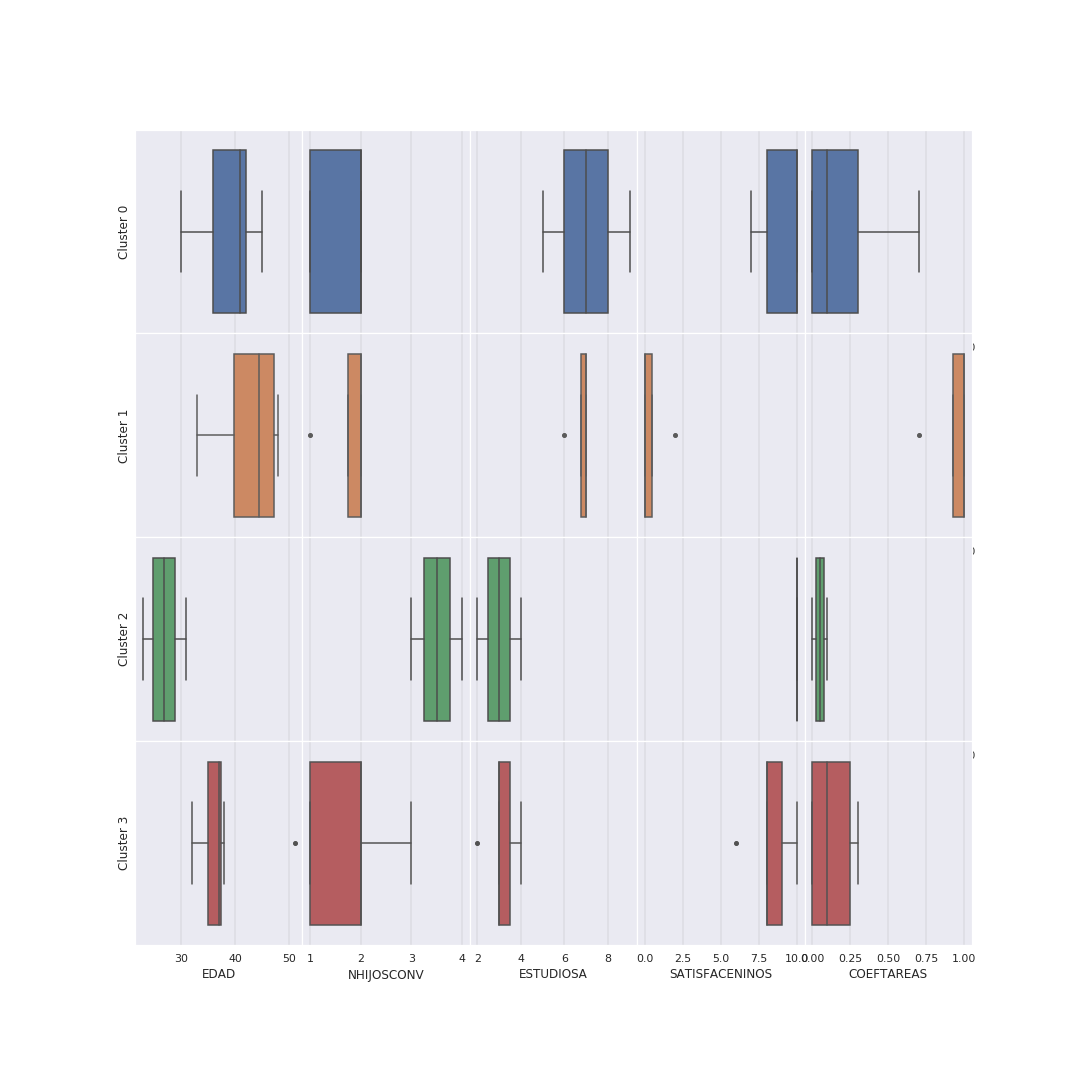
\includegraphics[scale=0.3]{../Caso3/homo/boxes}
		\caption{Caso 3: Distribución de variables en \emph{BoxPlot} para cada cluster, para parejas homosexuales.} 
		\label{boxes3homo}
	\end{figure}

	\begin{figure}[] 
		\centering
		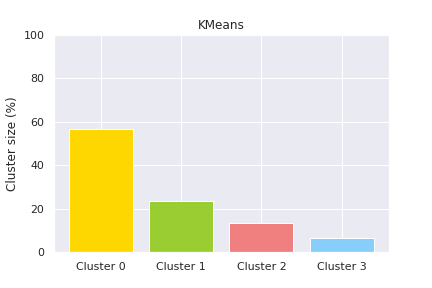
\includegraphics[scale=0.6]{../Caso3/homo/clusters}
		\caption{Caso 3: Tamaños de clusters para parejas homosexuales, fijado el algoritmo \emph{KMeans}} 
		\label{clusters3homo}
	\end{figure}
	
	\begin{figure}[] 
		\centering
		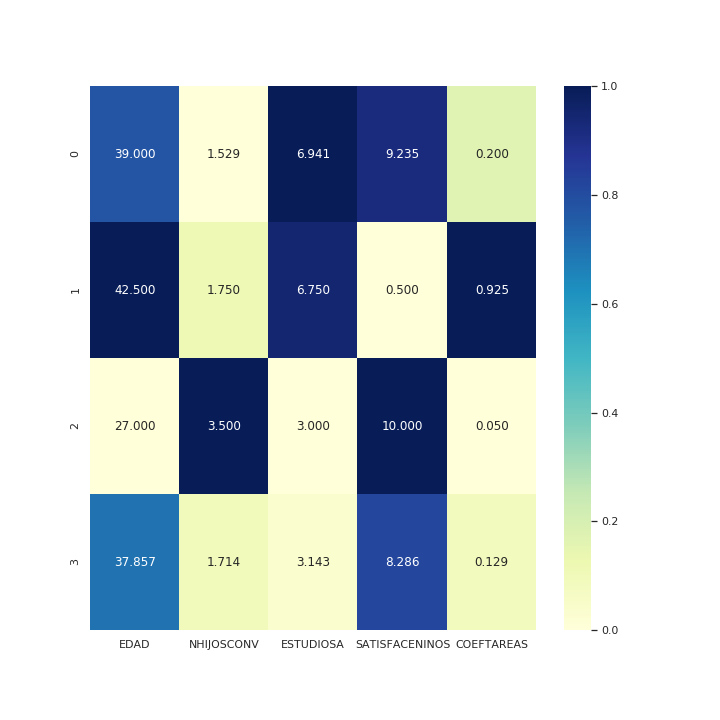
\includegraphics[scale=0.6]{../Caso3/homo/heatmap}
		\caption{Caso 3: \emph{HeatMap} de centroides para parejas homosexuales.} 
		\label{heatmap3homo}
	\end{figure}
	
	\begin{figure}[] 
		\centering
		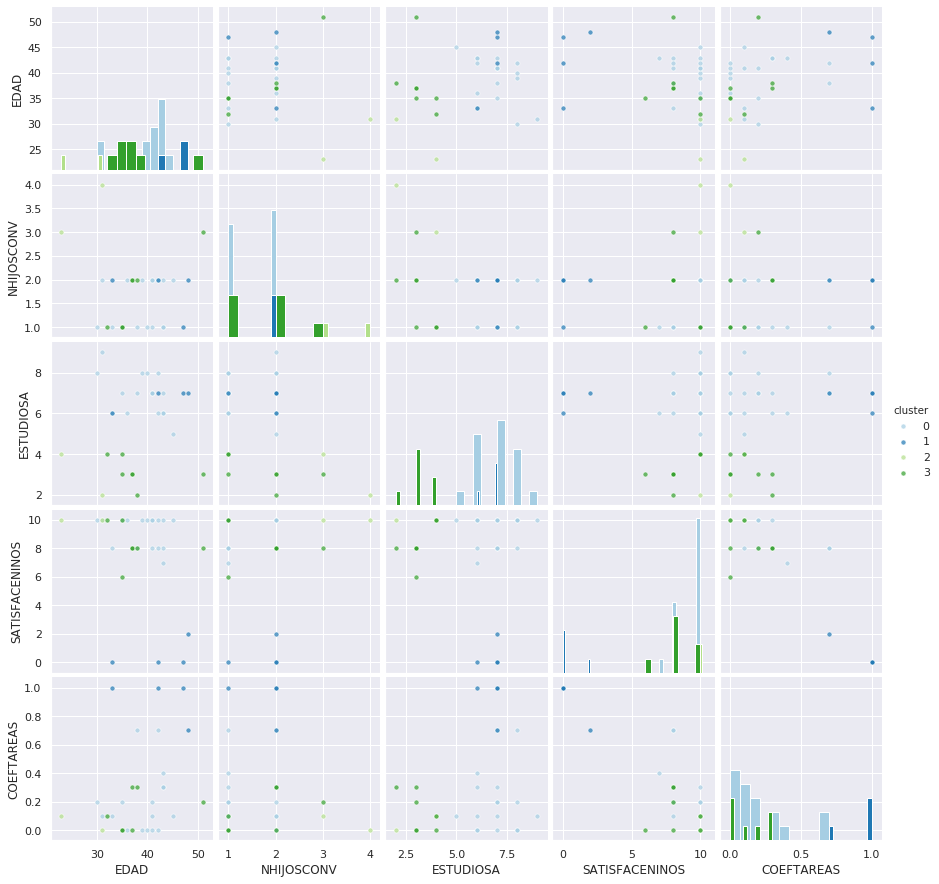
\includegraphics[scale=0.5]{../Caso3/homo/scatter_matrix}
		\caption{Caso 3: \emph{ScatterMatrix} para parejas homosexuales.}
		\label{scattermatrix3homo}
	\end{figure}
	
	\section{Bibliografía}
	\begin{thebibliography}{9}
		
		\bibitem{encuesta}
		Encuesta realizada por el Instituto Nacional de Estadística (INE) de donde obtenemos los datos.
		\href{https://www.ine.es/dyngs/INEbase/es/operacion.htm?c=Estadistica_C&cid=1254736177006&menu=ultiDatos&idp=1254735573002}{www.ine.es/dyngs/INEbase/es/operacion.htm?c=Estadistica\_C\&cid=1254736177006\& menu=ultiDatos\&idp=1254735573002}
		
		\bibitem{matplotlibDocumentation}
		Matplotlib API documentation.
		\href{https://matplotlib.org/contents.html}{matplotlib.org/contents.html}
		
		\bibitem{sklearnDocumentation}
		Scikit Sklearn API documentation.
		\href{https://scikit-learn.org/stable/modules/classes.html#module-sklearn.cluster}{scikit-learn.org/stable/modules/classes.html\#module-sklearn.cluster}
		
	\end{thebibliography}
	
\end{document}